\section{The GRANDProto35 detection unit} 
\label{feu}
Here we give a brief description of the structure of the GRANDProto35 detection unit and provide informations needed to make sure it runs in a proper state and identify possible problems when encountered. 

\subsection{Antenna}
{\bf To be done}

\subsection{Electronic Box Set-Up}
The electronic Box (EB) should be fixed to its antenna pole as shown in Fig. \ref{fig:casing}: the front pannel is vertical, with the pressure valve facing ground. The box may be fixed inside the lower vertical arm of the antenna. 

\begin{figure}[t!]
\begin{center}
{
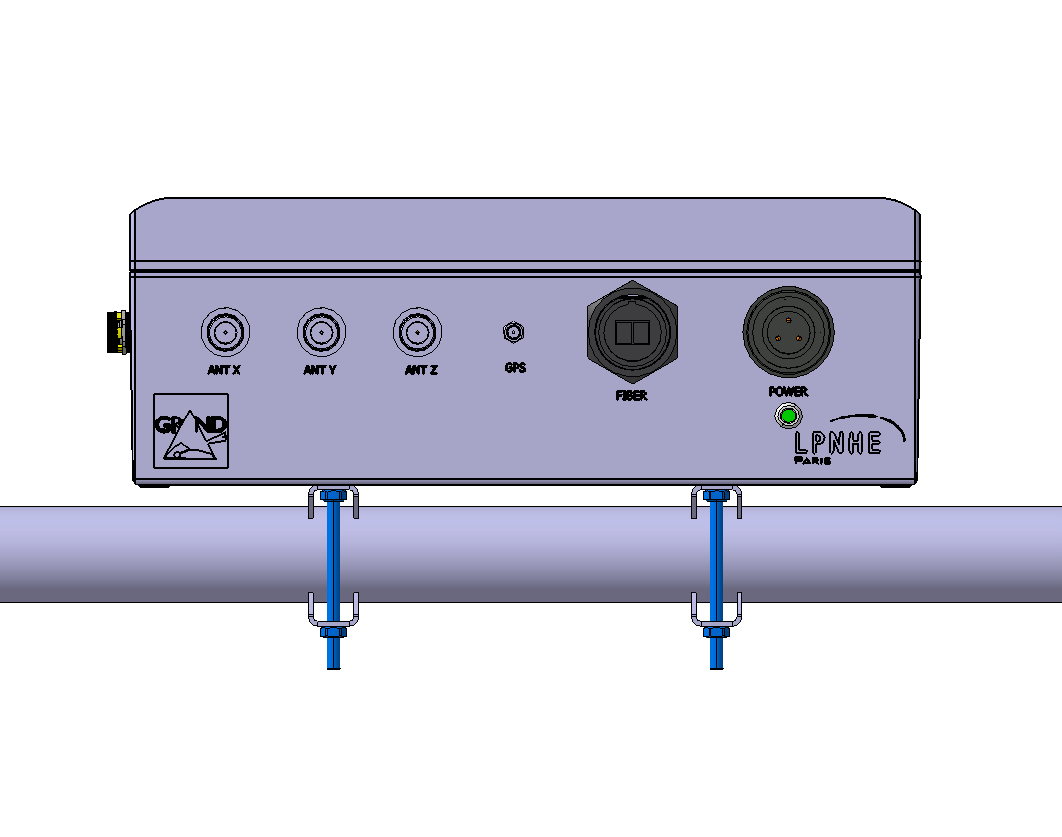
\includegraphics[width=6.5cm,angle=90]{plots/casing.jpg}  
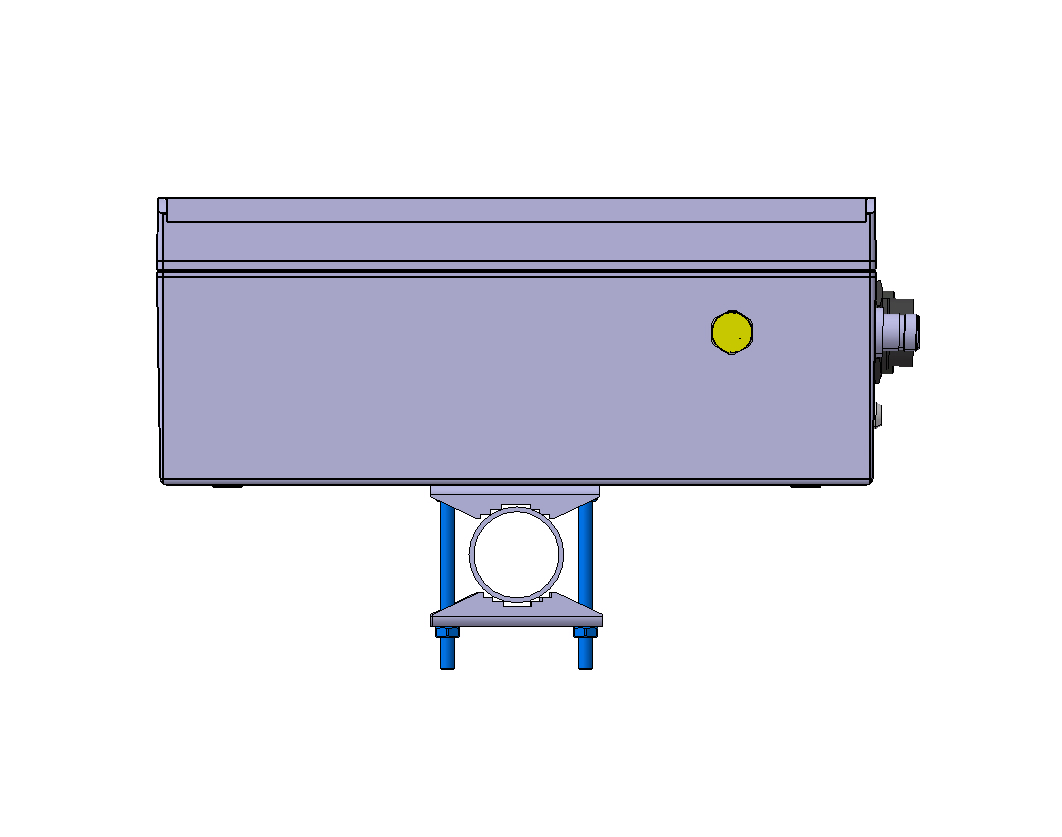
\includegraphics[width=6.5cm,angle=90]{plots/casing_bottom.jpg} 
}
\end{center}
\caption{Front (left) and bottom (right) views of a GRANDProto35 Electronic Box casing once fixed to an antenna pole. 
}
\label{fig:casing} 
\end{figure}


\subsection{Connections}
\label{connection}
Connections to the EB should be carried out in the following order:
\begin{enumerate}[i)]
\item {First connect the three outputs of the antenna to the associated inputs {\it ANT X}, {\it ANT Y}, {\it ANT Z} of the EB with the three dedicated 75$\Omega$ coaxial cables. \hl{Make sure here that you connect the 75$\Omega$ N-type connector end (the thinner one), and not the 50$\Omega$ one (thicker). Inversion would destroy the plug}. Also note that there is a 12\,V DC level on these cables, which is used to power the antenna LNAs (see section \ref{analog} for details). It is therefore safer to plug/unplugg them only when the EB power is off, in order to avoid possible short-cuts. 
}
\item {Then connect the GPS antenna. \hl{By no means should the GPS antenna be connected when the power is on}. This may destroy the GPS unit inside the board (see section \ref{digital}) and make it unusable. The GPS antenna should preferably be placed above ground. A magnet inside the GPS antenna allows to fix it to a close-by metalic surface. }
\item {Then connect the optical fiber (which can however be plugged/unplugged at any time, with no risk of damage). }
\item {Finally plug the power cable. Nominal value of the power supply should be 15\,V, but values between 9 and 20\,V are still OK. A green LED on the front panel just below the power plug allows to check if the board is powered on.}
\end{enumerate}

Cables between the box and the antenna should be tied to the pole to avoid dangling and stress on the connectors.

\subsection{Electronic Board description}
A picture of the board is shown in figure \ref{fig:board}. It can be divided in 4 functionnal sections: analog, digitial, communication and power supply.

\begin{figure}[t!]
\begin{center}
{
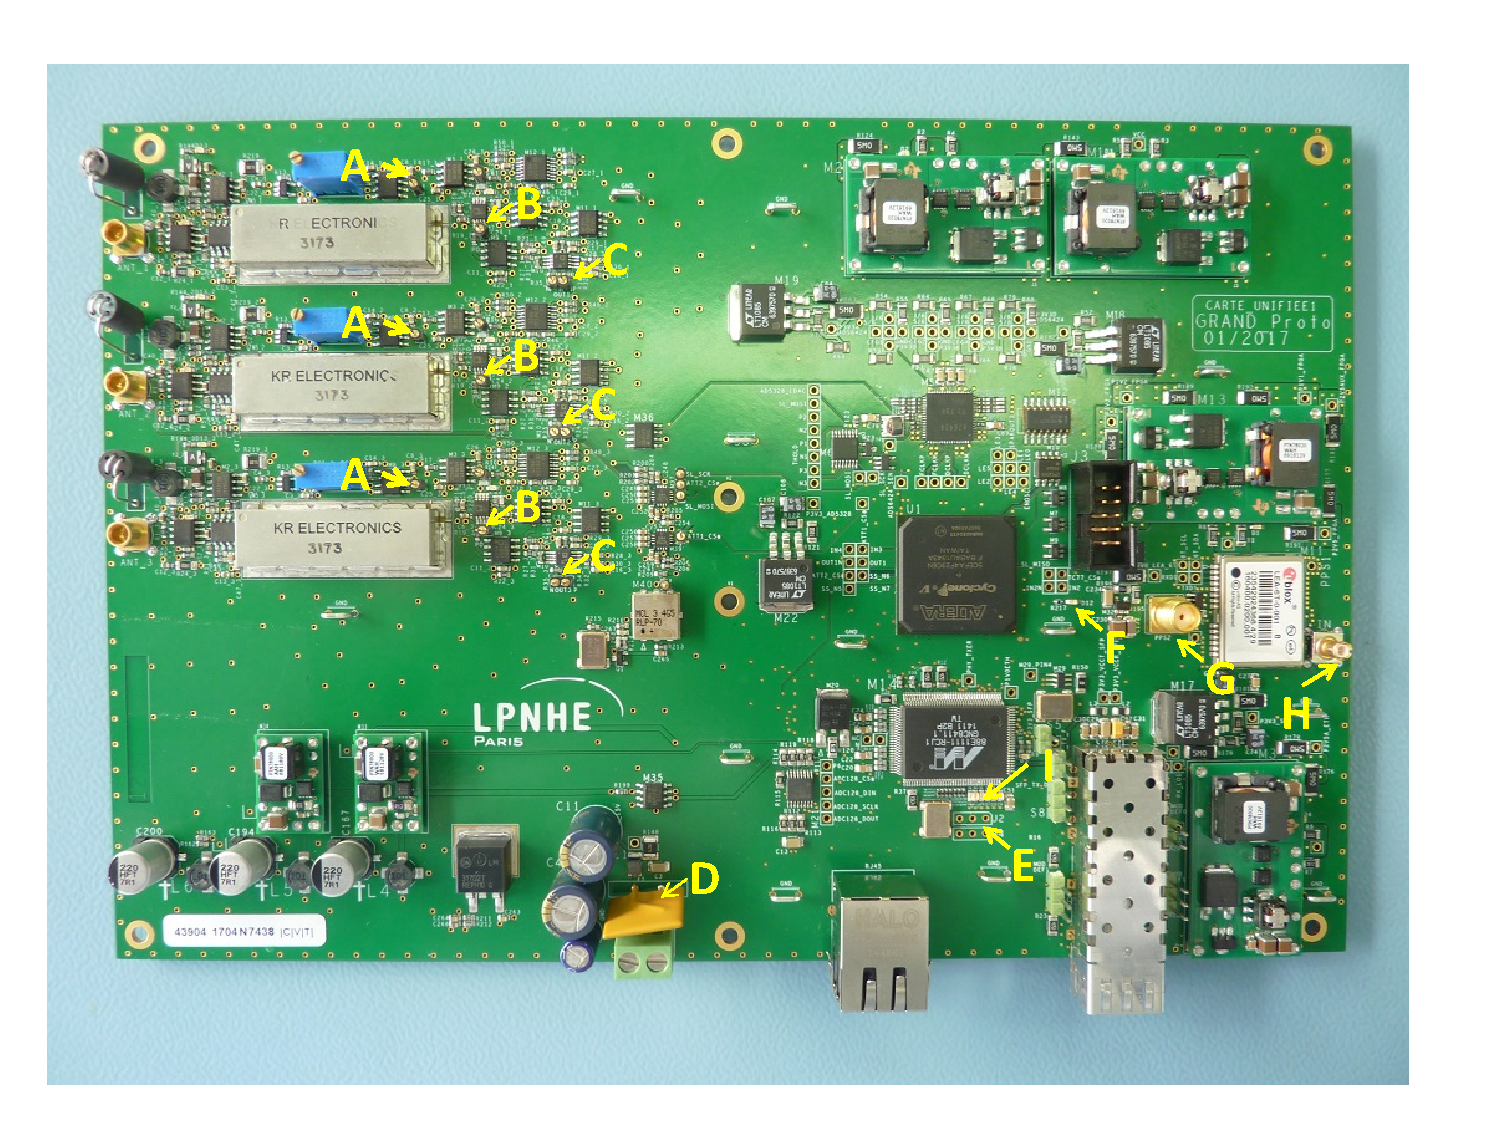
\includegraphics[width=\textwidth]{plots/GP35_FEU.pdf}  
}
\end{center}
\caption{Picture of the GRANDProto35 Electronic Board. Meaning of the letter tags: "A" stands for the measurement point for the the power dectector common-mode voltage level. The screw on the blue) potentiometer can be used to adjust the voltage value. "B": measurement point for the signal at output of the power detector. "C": differential measurement points for the signal at input of the ADC. "D": re-amarable fuse for board power input (see text for details). "E": jumper to switch between ethernet plug (left position) or optical (right position). "F": FPGA configuration flag, should lit in red when FPGA is properly configured. "G": GPS PPS signal output: should deliver a periodic pulse (T=1\,s) when GPS is properly set. "H": connector to the GPS antenna. "I": light signals for communication with board. {\bf specify here normal beahaviour}  
}
\label{fig:board} 
\end{figure}


\subsubsection{Analog part}
\label{analog}
The description of the analog part of the board is given in details in \cite{GP35ana} (in French). Here we just give a brief overview. \\
%
The analog part lies in the top-left corner of the board. Signal input to the board is done for each of the three channels through an MMCX 75$\Omega$ jack connected to the corresponding N-type connector. From top to bottom we have X, Y and Z channels. The signal is adapted to a 50$\Omega$ impedance thanks to a dedicated amplifier (G=4) placed just after the connector, then fed into the 30-100\,MHz filters tagged {\it KR ELECTRONICS}. Signal is finally processed through a power detector AD8310 \cite{AD8310}, which acts as an envelop detector. The power detector runs in differential mode. Its common mode voltage has a nominal value of 0.9\,V adjusted thanks to a potentiometer (blue square, just above the filter). The common-mode level can be measured between ground and the test point shown on Fig. \ref{fig:board} by the letter tag "A". \\
%
The analog section also provides the power supply to the LNAs placed inside the antenna nut through a bias-tee system implemnted in the analog section. \hl{This means that in normal operation, a 12\,V DC voltage is applied on the input plugs, which the user should be aware of when performing tests on a powered board.} Note however that the LNAs power supply can be switched on and off by the user using the remote command program (see section \ref{TRENDDAQ}).  \\
%
In addition to this, the analog part includes a trigger section, where the signals at the output of the filters are first amplified by an additionnal factor 10 thus bringing the total amplification for the trigger channel to $4 \times 10 = 40$. The signal level is then compared to threshold values set by the user through the remote control program. A trigger flag is generated and sent to the FPGA (see section \ref{digital}) if one channel exceeds it. Note that there are six independant trigger channels, corresponding to two polarities for each of the three channels. The user can activate/inhibit independantly each of these trigger channels and set their respective threshold values, again through the remote control program (see section \ref{TRENDTRIG}). \\
%
Finaly an internal calibration system is also included in this analog part: its core is a 66.6660\,MHz quartz oscillator (placed at the center of the board), which generates a sine wave. Its amplitude can be moderated thanks to two attenuators, with attenuation values adjustable by the user (see section \ref{TRENDDAQ}). When the user uses the DAQ in calibration mode, the input of the signal treatment chain detailed above is switched from the MMCX connector input to this calibration signal. This allows to calibrate the full DAQ chain. 
   

\subsubsection{Digital part}
\label{digital}
The digital treatment of the signal is detailed in \cite{GP35daq}. It is performed on the right part of the card, starting with a 4-channels ADC \cite{ADCdoc} running at a nominal frequency of 50\,MHz, ajustable up to 100\,MHz through the FPGA firmware. The ADC continously digitizes the signal coming from the three analog channels on 12 bits and within a dynamic range [-1\,V,+1\,V]. The 4$^{th}$ ADC channel is used in calibration mode to digitize the signal at the output of the quartz oscillator. It delivers dummy data in other run modes. The digital signal of each of the four channels is buffered in a circular register inside the FPGA. When one trigger is received (see previous section), a subset of length 2$\times${\it OFFSET} (where {\it OFFSET} is a parameter set by the user at run start) is saved for each of the four channels to form one event, with the trigger position being usually few samples after the middle position (index 105 for 180 samples). A GPS time-tag is also build  by the FPGA (see section \ref{timing}) and embeded in the event header and sent to the board output (see section \ref{comms}).

\subsubsection{Timing}
\label{timing}
A resolution of the order of 10\,ns on the antenna trigger time is requested in order to achieve a $\sim1^{\circ}$ resolution on the reconstructed direction of origin of the radio wave. The trigger time tagging in GRANDProto35 is done in the following way: 
\begin{enumerate}[-]
\item{the GPS unit delivers a pulse-per-second (PPS) signal to the FPGA. If the position of the GPS unit is known with good precison ($<$1\,m), a resolution of the order of 10\,ns is achievable on the PPS period (see \cite{GPS}). However the EB design only allows for a very basic communication with the GPS receiver, and the information on its true position cannot be provided to the GPS (note that similarly, no information other than the PPS signal can be retrieved from the GPS). The position of the GPS unit is therefore taken as its averaged value, provided the rms of its measurement do not exeed 10\,m. \hl{In case this condition is not reached, then no PPS signal is emitted}. So far however the timing info has always been present in the data after a few minutes, meaning that the PPS signal was indeed emitted. The actual timing precision achieved through this method is still to be determined.} 
\item{A counter inside the FPGA, running at a nominal 125\,MHz frequency, then provides a 8-ns granularity on the trigger time. The counter is reset at each new PPS signal. The counter value is a 32-bits integer named $TS2$, available in the header of the event data sent to the DAQ (see section \ref{format}). Note however that the counter frequency is not stable, and depends in particular on its temperature. In order to get a reliable time tag from the counter, the actual number of clock counts achieved between two PPS signals is recorded by the FPGA every second. This information is available in the slow control data (see section \ref{slc}), under the name {\it MAXCOARSE}.} 
\item{Additionnaly two more fields ($TS1PPS$ and $TS1Trigger$)  provide a nanosecond granularity of the time tag.} 
\end{enumerate}

Eventually, the absolute time tag for a trigger can be computed as~:
$$
t = t_0+\left(TS2+\frac{TS1PPS-TS1Trigger}{4}\right)\frac{1}{MaxCoarse} 
$$
where $t_0$ is the UTC second in which the trigger was received and the second term of the addition corresponds to the time elapsed between the beggining of that specific UTC second and the trigger. In order to compute $t_0$, the $SSS$ info is is used. Its raw value corresponds to the number of seconds since the board received its first PPS signal. As their GPS units may not start issuing the PPS signal at the same instant, there may be offsets between SSS values for different EBs. The SSS fields are therefore corrected online in the DAQ program, based on the DAQ unit GPS time info.


\subsubsection{Communication}
\label{comms}
Communication with the DAQ computer is done through a Marvell interface chip, using the GEDEK Communication Engine. Messages are exchanged using UDP protocol. Either a standard ethernet plug can be used, or optical transfer through an SFP connector. A jumper placed just below the Marvell chip allows to switch from one to the other (left: ethernet plug, right: optical, see letter tag "E" in Fig. \ref{fig:board})). The latter is the standard communication system in GRANDProto35 operation, with a bi-modal SFP ($\lambda_1$ = 1310\,nm \& $\lambda_2$ = 1550\,nm) allowing downstream (data) and upstream (commands) communication on one single fiber. \\
%
The EB is identified through a unique MAC adress given by a specific chip (Dallas DS2502). At boot time, IP adresses of all units are identically set to 192.168.1.18 by default.  A software program however allows to map each MAC adress to an IP adress of format 192.168.1.1xx (see section \ref{startup}) where xx is the EB ID, ranging between 01 and 35. This IP adress is used for any further communication with the DAQ PC, whose IP should be 192.168.1.10 within a local network (submask 255.255.255.0).


\subsubsection{Power supply}
The nominal power supply of the EB is 15\,V DC, but powers ranging between 9 and 30\,V are acceptable. The standard power consumption is $\sim$10W in normal run conditions. In standard operation at Ulastai, this DC voltage is provided by the external AC/DC converter installed at the pod level. There is also an internal AC/DC converter fixed on the internal side of the EB casing, but it is not used. \\
%
A re-armable fuse is installed at the input of the board power supply (letter tag "D"  on Fig. \ref{fig:board}). It will disrupt power supply in case a current surge is detected ({\bf level ?}). It is re-armed after power cycling. \\
%
DC voltages of +4\,V and -3.3\,V are generated by DC-DC converters located on small mezanines placed at 3 corners of the board.


\subsubsection{Slow control}
\label{slc}
Various slow-control parameters are measured on the board, and available for the user upon request (see section \ref{slcdaq}). In particular various key voltage values are monitored (master board voltage, +4\,V, -3\,V and LNA power suplies), as well as the temperature on the board. 

\subsubsection{Board control}
\label{control}
There are several tools to check that the board is in a proper state and identify possible issues. {\bf To be completed.}
